\chapter{Diseño}
\label{cap:diseno}

Este capítulo presenta el diseño del sistema desarrollado en este proyecto. Este capítulo se centra en el
\emph{qué} y el \emph{por qué} de cada diseño, no en el \emph{cómo} se ha implementado, que se detalla en el capítulo~\ref{cap:implementacion}.

\section{Arquitectura general}
\label{sec:diseno-arquitectura}

Como se avanzó en el capítulo~\ref{cap:analisis}
(Figura~\ref{fig:analisis-contexto}), el sistema se organiza en dos bloques
muy distintos: un \textbf{pipeline offline} en Python, y una \textbf{aplicación web} de visualización
que consume los resultados ya calculados. La
Figura~\ref{fig:diseno-arquitectura} representa esta arquitectura a nivel de
componentes: no las funcionalidades concretas de cada fase --eso se detalla
en las secciones siguientes de este capítulo--, sino los grandes bloques del
sistema y cómo se comunican entre sí.

\begin{figure}[htp]
\centering
\begin{tikzpicture}[
  every node/.style={align=center, font=\footnotesize},
  box/.style={draw, rounded corners, fill=blue!8, minimum width=3.4cm, minimum height=1.1cm},
  arrow/.style={-{Latex[length=2.5mm]}, thick}
]
\node[box, fill=gray!12] (dataset) {SoccerNet-Tracking\\(dataset externo)};
\node[box, right=1.6cm of dataset] (pipeline) {Pipeline offline\\(Python)};
\node[box, below=1.3cm of pipeline, minimum width=5.2cm, fill=yellow!12] (storage) {Artefactos persistidos en disco\\\footnotesize\texttt{.txt / .csv / .png / .mp4 / .json}};
\node[box, right=1.6cm of pipeline, fill=orange!10] (web) {Aplicación web\\(React + Vite + TS)};
\draw[arrow] (dataset) -- (pipeline) node[midway, above, font=\tiny] {\texttt{det.txt}, \texttt{gt.txt}};
\draw[arrow] (pipeline) -- (storage);
\draw[arrow] (storage) -- (web) node[midway, above, font=\tiny, sloped] {paquete exportado};
\draw[arrow] (storage.north) to[out=100, in=260] node[midway, left, font=\tiny] {reanuda desde cualquier fase} (pipeline.south);
\end{tikzpicture}
\caption{Arquitectura general del sistema, a nivel de componentes: el
pipeline offline persiste todo su trabajo en disco en vez de mantener
estado en memoria, y la aplicación web consume ese mismo almacenamiento ya
calculado, sin recalcular nada ni compartir proceso con el pipeline.}
\label{fig:diseno-arquitectura}
\end{figure}

Esta arquitectura por artefactos persistidos tiene tres ventajas de diseño
aprovechadas en este proyecto. Primero, permite
\textbf{reanudar} el trabajo desde cualquier fase sin repetir las
anteriores: el estudio de hiperparámetros (sección~\ref{sec:diseno-hiperparametros})
se apoya en resultados de tracking ya calculados, y el pipeline de
metadatos (sección~\ref{sec:diseno-metadatos}) se apoya en la configuración
óptima ya validada, sin necesidad de volver a ejecutar el tracking desde
cero cada vez. Segundo, favorece la \textbf{reproducibilidad}
(RNF-001): cualquier resultado puede auditarse inspeccionando el artefacto
correspondiente. Tercero,
es la base que permite a la aplicación web
(sección~\ref{sec:diseno-web}) limitarse a consumir artefactos estáticos.

\section{Diseño del pipeline de tracking}
\label{sec:diseno-tracking}

El pipeline de tracking transforma las detecciones precomputadas de una
secuencia en trayectorias con identidad consistente,
aplicando el algoritmo de tracking correspondiente
(sección~\ref{sec:fundamentos-algoritmos}). Se compone de tres bloques de
diseño: el filtrado del balón, la ejecución del algoritmo de tracking sobre
una única secuencia, y la orquestación de esa ejecución sobre la totalidad
de un split.

\subsection{Diseño del filtrado del balón}
\label{subsec:diseno-balon}

Como se justificó en la sección~\ref{subsec:fundamentos-balon}, el balón se
separa de las detecciones de personas mediante un filtro geométrico, no
mediante un detector entrenado. El diseño de este filtro es deliberadamente
simple: para cada detección del frame, se evalúan dos condiciones
independientes sobre su caja delimitadora: su área en píxeles y su
proporción ancho/alto, y solo si ambas se cumplen a la vez la detección
se aparta del flujo de tracking de personas, como ilustra la
Figura~\ref{fig:diseno-balon}. Los valores concretos de los dos umbrales
empleados se detallan y justifican en la
sección~\ref{sec:implementacion-tracking}.

\begin{figure}[htp]
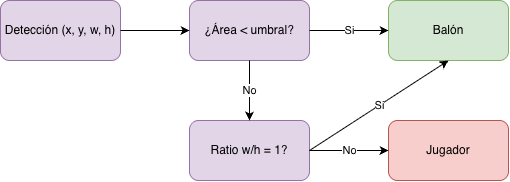
\includegraphics[width=0.85\textwidth]{figures/disenobalon.drawio.png}
\caption{Diseño del filtro geométrico de separación del balón: dos
condiciones sobre área y proporción de la caja delimitadora, evaluadas
sobre cada detección de cada frame antes de invocar al tracker.}
\label{fig:diseno-balon}
\end{figure}

\subsection{Diseño de los algoritmos de tracking}
\label{subsec:diseno-tracking-algoritmos}

Los dos algoritmos comparados (ByteTrack y OC-SORT)
se ejecutan a través de la interfaz común que expone la librería
\texttt{boxmot} (sección~\ref{sec:analisis-decision}), lo que permite que el
diseño del bucle principal de procesamiento sea idéntico para ambos y solo
cambie la clase de tracker instanciada. Este diseño responde directamente al
requisito de extensibilidad (RNF-004): incorporar un tercer algoritmo
disponible en \texttt{boxmot} no exige rediseñar el bucle, solo
instanciarlo. La Figura~\ref{fig:diseno-tracking-loop} representa este
bucle, común a ambos algoritmos.

\begin{figure}[htp]
\centering
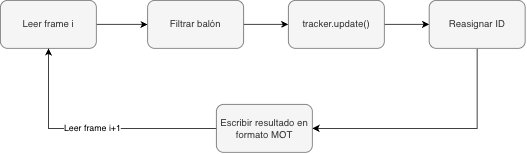
\includegraphics[width=0.85\textwidth]{figures/diseno_trackers.drawio.png}
\caption{Bucle de procesamiento común a ambos algoritmos de tracking.}
\label{fig:diseno-tracking-loop}
\end{figure}

El paso de \textbf{reasignación de identificador} merece un diseño propio:
los algoritmos de \texttt{boxmot} generan identificadores internos
arbitrarios y no necesariamente consecutivos, mientras que el formato MOT
esperado por \texttt{TrackEval} y por la interpretación humana de los
resultados es más claro con una numeración secuencial 1..N por secuencia.
El diseño mantiene, por tanto, una tabla de correspondencia
\emph{identificador interno del tracker} $\to$ \emph{identificador
secuencial}, poblada de forma que cada vez que se encuentra un nuevo
identificador interno, se le asigna el siguiente número secuencial
disponible.

\subsection{Diseño de la ejecución batch sobre un split completo}
\label{subsec:diseno-batch}

Ejecutar manualmente cada algoritmo sobre cada una de las secuencias de un
split sería inviable en la práctica y,
sobre todo, propenso a inconsistencias entre secuencias (parámetros
distintos por descuido, secuencias olvidadas). El diseño de la ejecución
batch resuelve esto con un orquestador que recorre automáticamente todas
las secuencias de un directorio de split, aplicando a cada una el mismo
bucle de la Figura~\ref{fig:diseno-tracking-loop} para cada uno de los
algoritmos configurados, como se representa en la
Figura~\ref{fig:diseno-batch}.

\begin{figure}[htp]
\centering
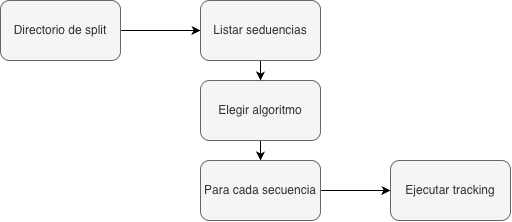
\includegraphics[width=0.85\textwidth]{figures/diseno_batch.drawio.png}
\caption{Diseño de la ejecución batch: doble bucle sobre algoritmos y
secuencias de un split, reutilizando el bucle de procesamiento de la
Figura~\ref{fig:diseno-tracking-loop} para cada combinación.}
\label{fig:diseno-batch}
\end{figure}

\section{Diseño de la evaluación}
\label{sec:diseno-evaluacion}

La evaluación traduce los resultados de tracking y el
\emph{ground truth} en las métricas de la
sección~\ref{sec:fundamentos-metricas}, delegando el cálculo en
\texttt{TrackEval} en lugar de reimplementar las métricas. El diseño de
esta fase se limita, por tanto, a preparar correctamente la entrada que
\texttt{TrackEval} espera y a configurar qué métricas calcular, como
resume la Figura~\ref{fig:diseno-evaluacion}.

\begin{figure}[htp]
\centering
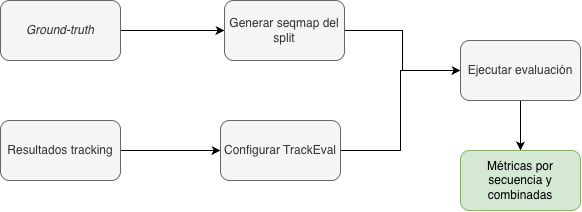
\includegraphics[width=0.85\textwidth]{figures/diseno_eval.drawio.png}
\caption{Diseño de la fase de evaluación.}
\label{fig:diseno-evaluacion}
\end{figure}

Un aspecto de diseño relevante, es que esta misma fase de
evaluación se ejecuta \textbf{dos veces con distinto propósito}: una
primera vez sobre el conjunto de entrenamiento, durante el desarrollo
inicial, y una segunda vez sobre el conjunto de test, cuyos resultados son los que finalmente se usan para las
conclusiones comparativas. El diseño
mantiene ambas ejecuciones completamente separadas.

\section{Diseño del estudio de hiperparámetros}
\label{sec:diseno-hiperparametros}

El estudio de hiperparámetros reutiliza el bucle de tracking
(Figura~\ref{fig:diseno-tracking-loop}) y la fase de evaluación
(Figura~\ref{fig:diseno-evaluacion}) como bloques ya diseñados, y añade
sobre ellos un bucle de búsqueda \emph{uno a uno}. La Figura~\ref{fig:diseno-hiperparametros} representa
este diseño.

\begin{figure}[htp]
\centering
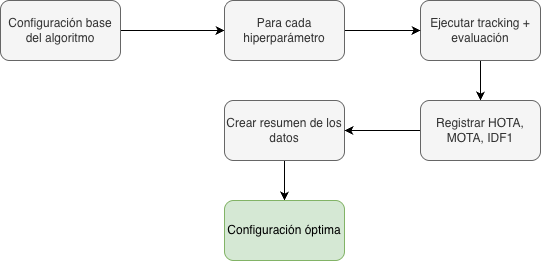
\includegraphics[width=0.85\textwidth]{figures/diseno_hiper.drawio.png}
\caption{Diseño del estudio de hiperparámetros: barrido uno a uno sobre el
conjunto de test, resumen comparativo y validación final de la
configuración óptima de cada algoritmo.}
\label{fig:diseno-hiperparametros}
\end{figure}

Este diseño es una decisión deliberada: una
búsqueda combinada crece exponencialmente con el número de parámetros y de
secuencias de test evaluadas en cada combinación, mientras que el barrido
uno a uno, con un coste lineal, permite \textbf{atribuir con
claridad} el efecto observado a un parámetro concreto, algo que
una rejilla combinada por ejemplo dificultaría al mezclar los efectos de varios
parámetros a la vez.

\section{Diseño del pipeline de metadatos}
\label{sec:diseno-metadatos}

El pipeline de metadatos parte de los resultados de tracking generados con
la configuración óptima de ByteTrack (determinada en la fase anterior) y
produce los cuatro tipos de metadatos deportivos de este proyecto. Como muestra la
Figura~\ref{fig:diseno-metadatos-dependencias}, estos cuatro bloques no son
independientes entre sí.

\begin{figure}[htp]
\centering
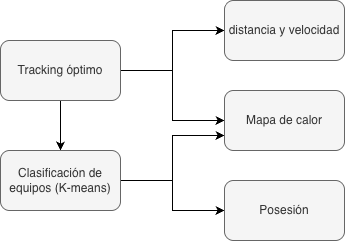
\includegraphics[width=0.85\textwidth]{figures/diseno_metadatos.drawio.png}
\caption{Dependencias entre los bloques del pipeline de metadatos.}
\label{fig:diseno-metadatos-dependencias}
\end{figure}

\subsection{Diseño de la clasificación de equipos}
\label{subsec:diseno-equipos}

La clasificación de equipos se diseña en dos niveles de K-means encadenados
(sección~\ref{sec:fundamentos-kmeans}), representados en la
Figura~\ref{fig:diseno-equipos}: primero, un K-means con $k=1$ extrae el
color dominante de la camiseta de \emph{cada} detección de jugador,
recortando la región central-superior de su caja delimitadora para evitar
incluir piernas, césped o balón en el recorte; después, un segundo K-means
con $k=2$ agrupa \emph{todos} los colores dominantes obtenidos, asumiendo
dos equipos con colores de camiseta distintos (RN-004). Por eficiencia, el
primer nivel no se aplica a todas las detecciones de la secuencia, sino a
un muestreo de frames, suficiente para determinar el equipo mayoritario de
cada \texttt{track\_id} sin procesar la secuencia completa.

\begin{figure}[htp]
\centering
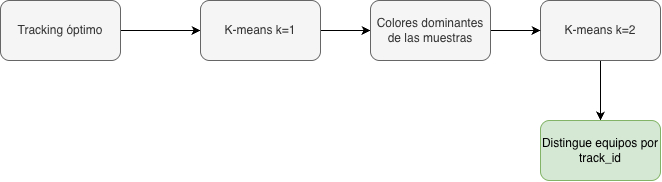
\includegraphics[width=0.85\textwidth]{figures/diseno_equipos.drawio.png}
\caption{Diseño de la clasificación de equipos: K-means en dos niveles.}
\label{fig:diseno-equipos}
\end{figure}

\begin{figure}[htp]
\centering
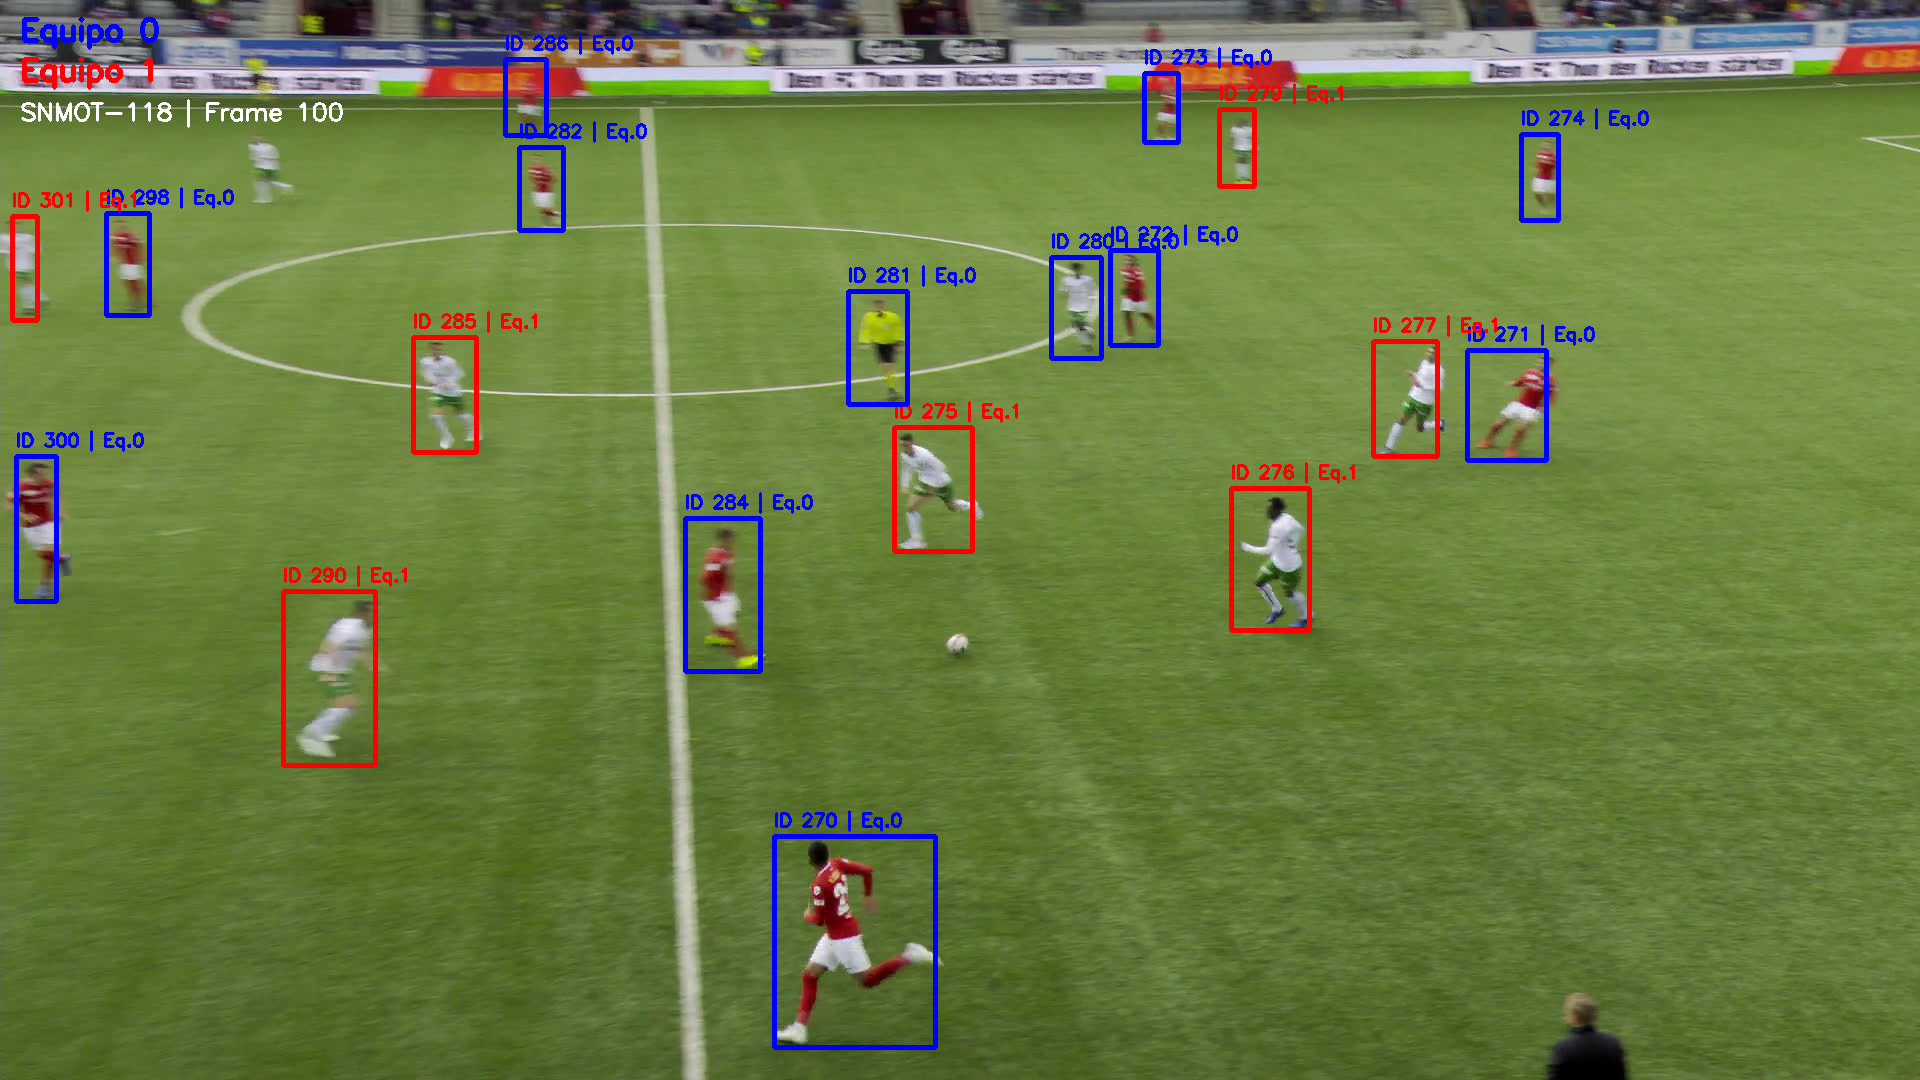
\includegraphics[width=0.85\textwidth]{figures/diseno_teams_ejemplo.png}
\caption{Resultado real de la clasificación de equipos sobre un frame de
SNMOT-118: cada jugador coloreado según el equipo asignado por K-means.}
\label{fig:diseno-teams-ejemplo}
\end{figure}

\subsection{Diseño de los mapas de calor}
\label{subsec:diseno-heatmaps}

Los mapas de calor de ocupación del campo se diseñan como una proyección de
las posiciones de tracking sobre un campo dibujado a escala
(Figura~\ref{fig:fundamentos-campo}), seguida de una estimación de densidad
por núcleos (\emph{Kernel Density Estimation}, KDE) que suaviza la nube de
puntos discretos en un mapa continuo. Se diseñan dos variantes, que
comparten el mismo procedimiento de proyección y KDE pero difieren en el
conjunto de posiciones de entrada: el mapa \textbf{general}, con todas las
posiciones de la secuencia, y el mapa \textbf{por equipo}
(sección~\ref{subsec:diseno-equipos}), que separa las posiciones según la
clasificación de equipos y usa la misma escala para ambos equipos, de modo
que sean directamente comparables entre sí.

\begin{figure}[htp]
\centering
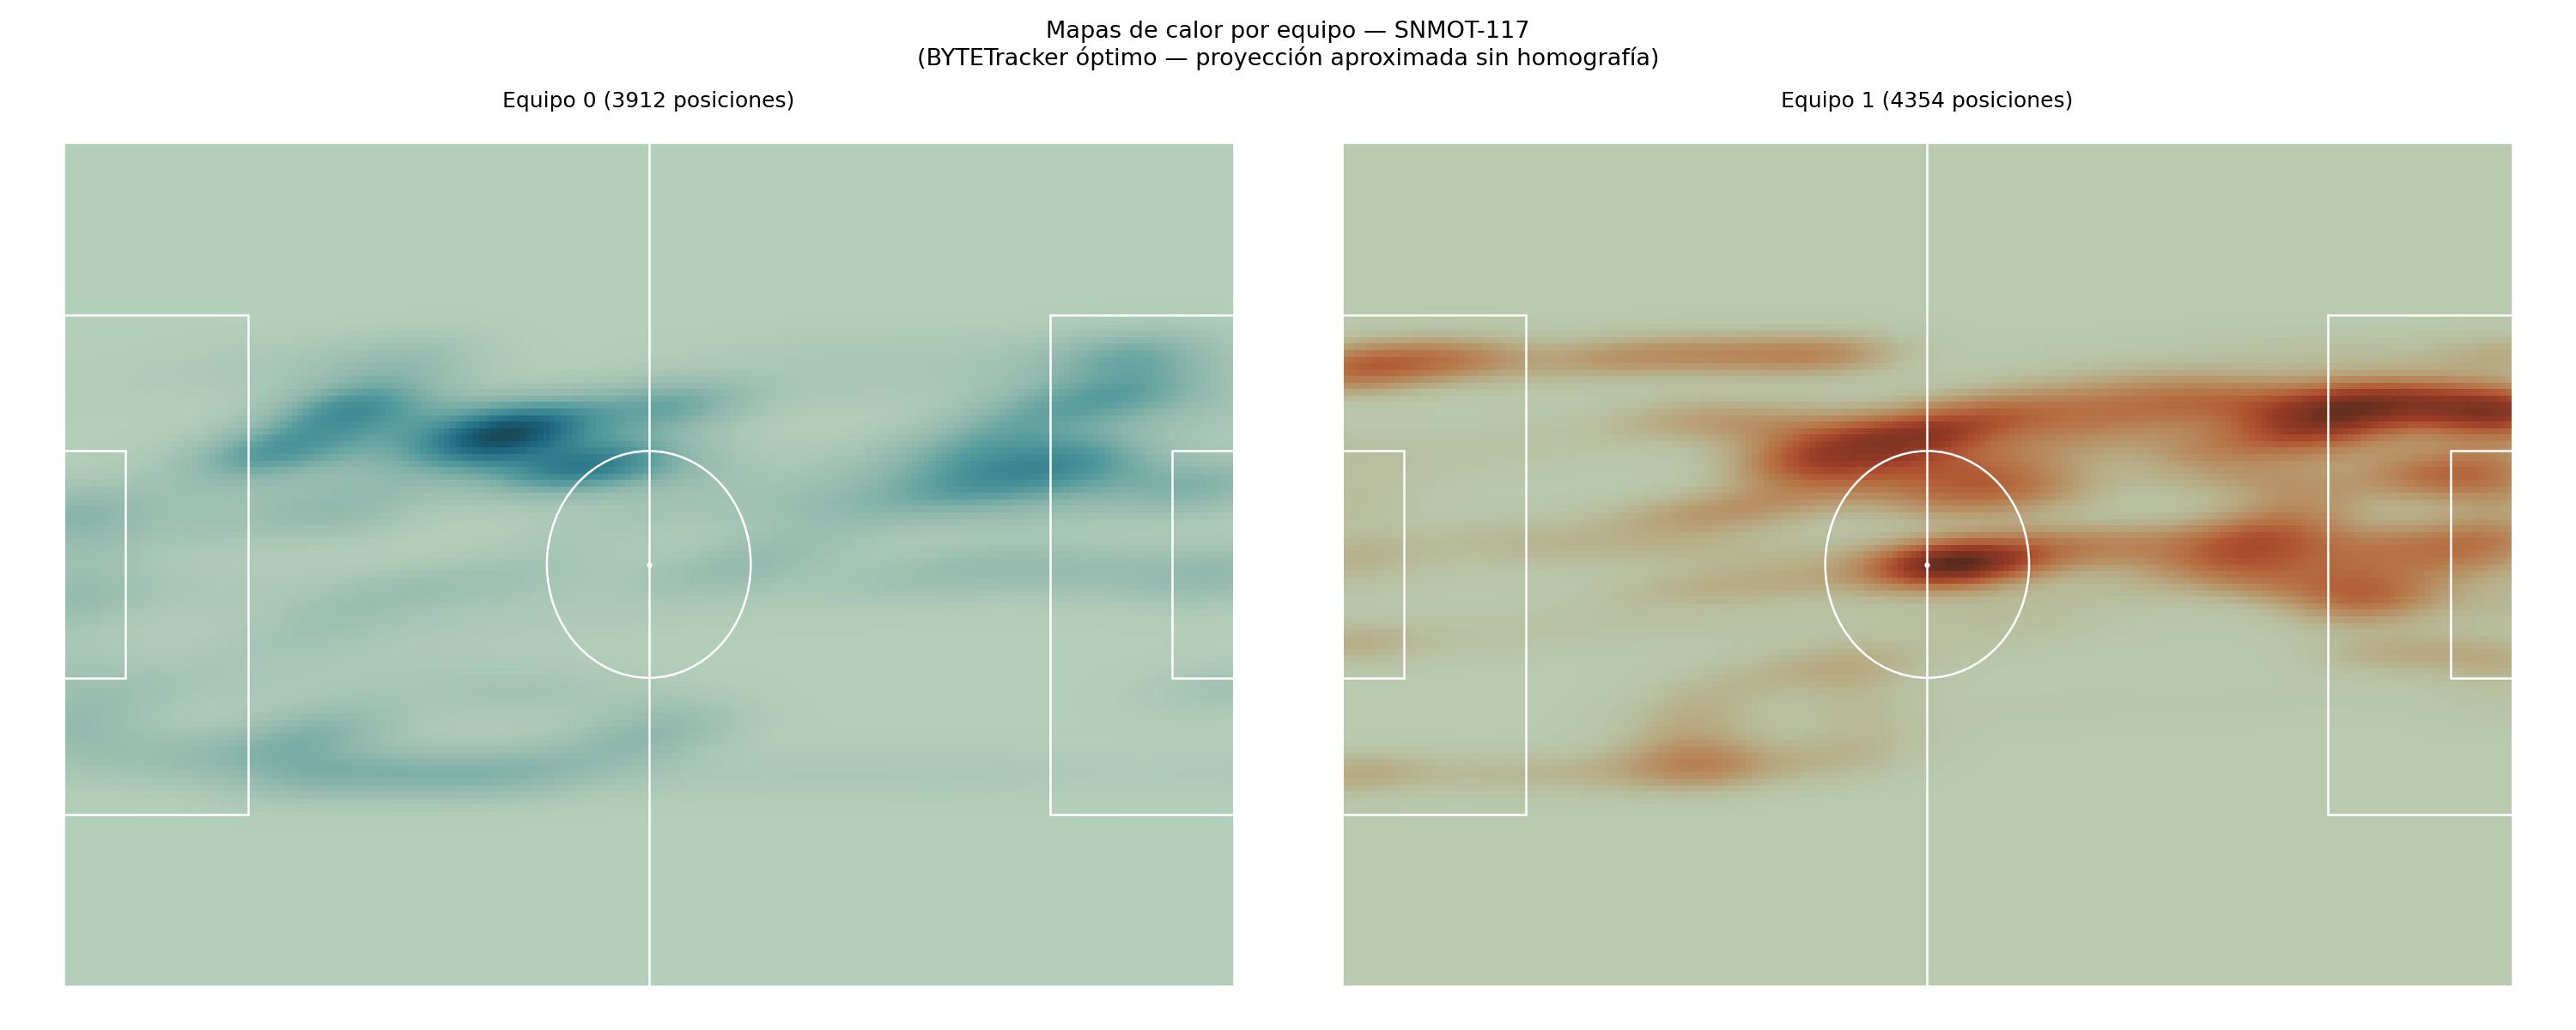
\includegraphics[width=0.95\textwidth]{figures/diseno_heatmap_by_team_ejemplo.png}
\caption{Resultado real del mapa de calor por equipo sobre SNMOT-117.}
\label{fig:diseno-heatmap-ejemplo}
\end{figure}

\subsection{Diseño de la homografía y la estimación de distancia/velocidad}
\label{subsec:diseno-homografia}

Como se explicó en la sección~\ref{sec:fundamentos-homografia}, este
proyecto distingue dos niveles de fiabilidad en la proyección de
coordenadas. El primero, usado de forma
general en los mapas de calor,
es una \textbf{proyección aproximada} que escala las posiciones observadas
por su rango directamente sobre las dimensiones del
campo. El segundo, diseñado como prueba
de concepto sobre un tramo concreto de cámara estable, es una
\textbf{homografía real}, calculada a partir de 4 puntos de referencia.
 La Figura~\ref{fig:diseno-homografia}
representa el diseño de este segundo nivel, el único que permite calcular
distancia y velocidad en unidades reales (RF-014).

\begin{figure}[htp]
\centering
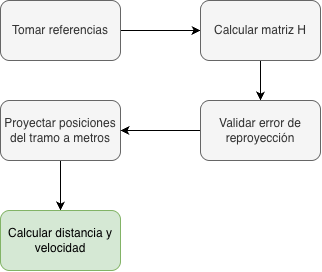
\includegraphics[width=0.85\textwidth]{figures/diseno_distancia.drawio.png}
\caption{Diseño de la homografía}
\label{fig:diseno-homografia}
\end{figure}

Un elemento de diseño importante, que se retoma como limitación en el
capítulo~\ref{cap:pruebas}, es que la zona del campo fuera del entorno
cercano a los 4 puntos de calibración no es fiable con esta homografía.
Figura~\ref{fig:diseno-heatmap-homografia-ejemplo}.

\begin{figure}[htp]
\centering
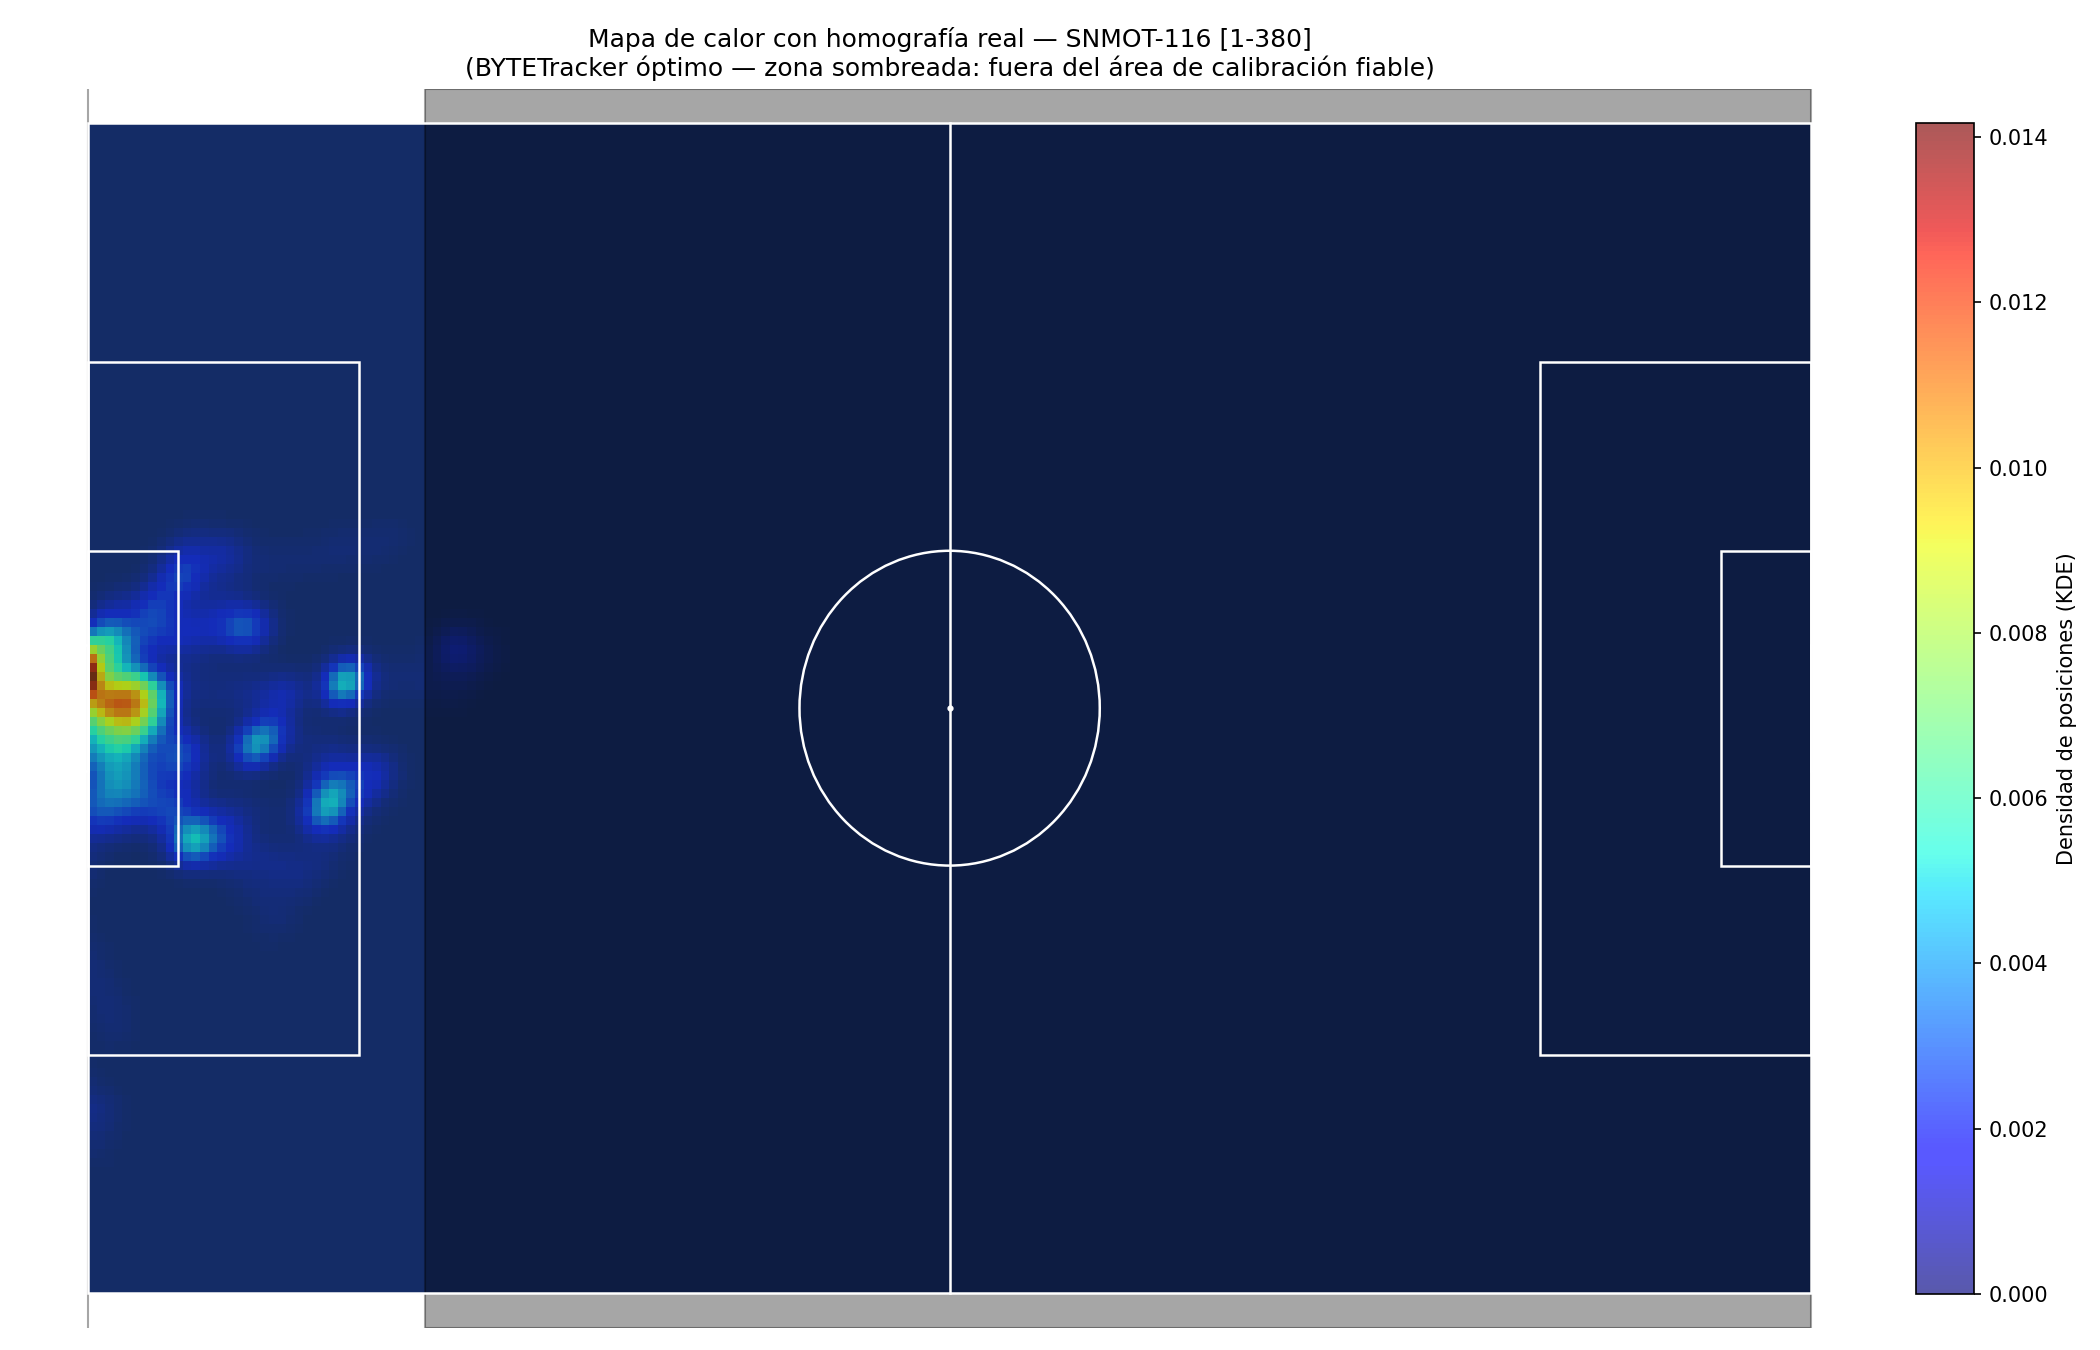
\includegraphics[width=0.85\textwidth]{figures/diseno_heatmap_homografia_ejemplo.png}
\caption{Resultado real del mapa de calor con homografía real sobre un
tramo de SNMOT-116.}
\label{fig:diseno-heatmap-homografia-ejemplo}
\end{figure}

\subsection{Diseño de la estimación de posesión}
\label{subsec:diseno-posesion}

La posesión de balón se diseña como una heurística de proximidad espacial
frame a frame. Para cada frame en que el filtro
geométrico (sección~\ref{subsec:diseno-balon}) detecta un balón, se calcula
la distancia entre su posición y la de todos los jugadores de ese frame; si
el jugador más cercano está por debajo de un umbral máximo de distancia, la posesión de ese frame se asigna a su equipo;
en caso contrario, se considera
balón suelto y el frame no cuenta para ningún equipo. La
Figura~\ref{fig:diseno-posesion} resume este diseño.

\begin{figure}[htp]
\centering
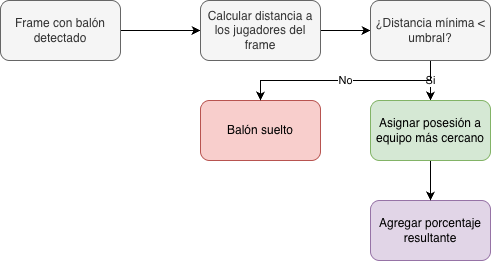
\includegraphics[width=0.85\textwidth]{figures/diseno_posesion.drawio.png}
\caption{Diseño de la estimación de posesión.}
\label{fig:diseno-posesion}
\end{figure}

\section{Diseño de datos y artefactos}
\label{sec:diseno-artefactos}

Como se ha señalado en la sección~\ref{sec:diseno-arquitectura}, el
contrato entre fases de este sistema son los artefactos que cada una
persiste en disco. La Tabla~\ref{tab:diseno-artefactos} cataloga estos
artefactos por fase, con su formato y su carpeta de salida.

\begin{table}[htp]
\centering
\caption{Catálogo de artefactos generados por cada fase del sistema.}
\label{tab:diseno-artefactos}
\renewcommand{\arraystretch}{1.2}
\small
\begin{tabular}{|p{2.9cm}|p{3.8cm}|p{1.5cm}|p{3.9cm}|}
\hline
\rowcolor{gray!25}
\textbf{Fase} & \textbf{Artefacto} & \textbf{Formato} & \textbf{Carpeta} \\
\hline
Tracking & Trayectorias por secuencia y algoritmo & \texttt{.txt} (MOT) &
  \texttt{results\_\allowbreak train/}, \texttt{results\_\allowbreak test/} \\
\hline
Evaluación & Métricas por secuencia y combinadas & \texttt{.csv},
  \texttt{.txt} & \texttt{evaluation\_\allowbreak train/}, \texttt{evaluation\_\allowbreak test/} \\
\hline
Hiperparámetros & Trayectorias y métricas por configuración & \texttt{.txt},
  \texttt{.csv} & \texttt{results\_\allowbreak hyperparam/},
  \texttt{evaluation\_\allowbreak hyperparam/} \\
\hline
Hiperparámetros & Tabla resumen y gráficas comparativas & \texttt{.csv},
  \texttt{.png} & \texttt{evaluation\_\allowbreak hyperparam/\allowbreak plots/} \\
\hline
Equipos & Muestras de color y asignación final por jugador & \texttt{.csv} &
  \texttt{metadata\_\allowbreak output/teams/} \\
\hline
Equipos & Visualización de la clasificación sobre un frame & \texttt{.png} &
  \texttt{metadata\_\allowbreak output/teams/} \\
\hline
Mapas de calor & Mapa general, por equipo y con homografía & \texttt{.png} &
  \texttt{metadata\_\allowbreak output/heatmaps/},
  \texttt{metadata\_\allowbreak output/\allowbreak heatmap\_\allowbreak homography\_\allowbreak demo/} \\
\hline
Homografía & Distancia y velocidad por jugador & \texttt{.csv} &
  \texttt{metadata\_\allowbreak output/\allowbreak distance\_\allowbreak homography\_\allowbreak demo/} \\
\hline
Posesión & Posesión por frame y resumen por equipo & \texttt{.csv} &
  \texttt{metadata\_\allowbreak output/\allowbreak possession/} \\
\hline
Exportación & Vídeos anotados & \texttt{.mp4} & \texttt{videos/} \\
\hline
\end{tabular}
\end{table}

\section{Diseño de la aplicación web}
\label{sec:diseno-web}

Esta sección presenta el diseño de la aplicación web, ya
implementada como parte de este proyecto. Se mantiene aquí, en el
capítulo de diseño, porque las decisiones arquitectónicas que se describen
a continuación se tomaron antes de programarla y se respetaron sin cambios
durante la implementación.

\subsection{Arquitectura de la aplicación web}

Siguiendo el mismo principio de artefactos persistidos de la
sección~\ref{sec:diseno-arquitectura}, la aplicación web se implementa como
una aplicación de una sola página (\emph{Single Page Application}, React +
Vite + TypeScript) que consume exclusivamente artefactos estáticos ya
exportados por el pipeline, sin ejecutar Python ni recalcular nada en el
navegador, ni base de datos, ni llamadas de red
más allá de peticiones \texttt{fetch} a ficheros JSON, PNG y MP4. 
Esta decisión, coherente con la arquitectura general del sistema, permite que
la interfaz se pueda desplegar en cualquier alojamiento estático (o
servirse en local).

Los artefactos que consume la aplicación no son los mismos ficheros
intermedios de la Tabla~\ref{tab:diseno-artefactos}, sino un paquete
derivado y empaquetado específicamente para la web por
\texttt{src/web\_export/export\_bundle.py}.

\begin{figure}[htp]
\centering
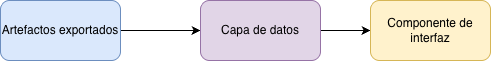
\includegraphics[width=0.85\textwidth]{figures/arquitectura_web.drawio.png}
\caption{Arquitectura de la aplicación web: los artefactos exportados por
\texttt{export\_bundle.py} alimentan una capa de datos (peticiones
\texttt{fetch} a JSON/PNG/MP4) que a su vez alimenta los componentes de
interfaz de React.}
\label{fig:diseno-web-arquitectura}
\end{figure}

\subsection{Diseño de la interfaz de usuario}
\label{subsec:diseno-web-ui}

La interfaz se organiza en dos pestañas, cada una centrada en una tarea
distinta: comparar el rendimiento agregado de los dos algoritmos, o
explorar en detalle los resultados de una secuencia concreta.

La pestaña \textbf{Comparativa de algoritmos} reproduce los resultados ya presentados en el
capítulo~\ref{cap:pruebas}: las tablas de HOTA/HOTA(0)/DetA/AssA/MOTA/IDF1
por \emph{split} (entrenamiento y test), la configuración óptima de
hiperparámetros de cada algoritmo, y las gráficas del estudio de
hiperparámetros y de la comparativa HOTA frente a HOTA(0).

La pestaña \textbf{Explorador de secuencias} (Figura~\ref{fig:diseno-web-wireframe})
está organizada en torno a una única tarea principal: seleccionar una
secuencia (SNMOT-116/117/118) evaluadas y un algoritmo (ByteTrack u OC-SORT)
mediante un selector, y explorar los resultados de esa
combinación.

No todas las combinaciones de secuencia y algoritmo tienen los mismos
datos disponibles: SNMOT-117 no tiene puntos de calibración de homografía
(sección~\ref{sec:implementacion-homografia}), y la combinación
ByteTrack/SNMOT-118 nunca llegó a generar un mapa de calor por equipo en
el pipeline original. La interfaz
muestra explícitamente una nota indicando que el dato no está disponible
para esa combinación, para que la ausencia se lea como una característica
real de los datos y no como un error de carga.

\begin{figure}[htp]
\centering
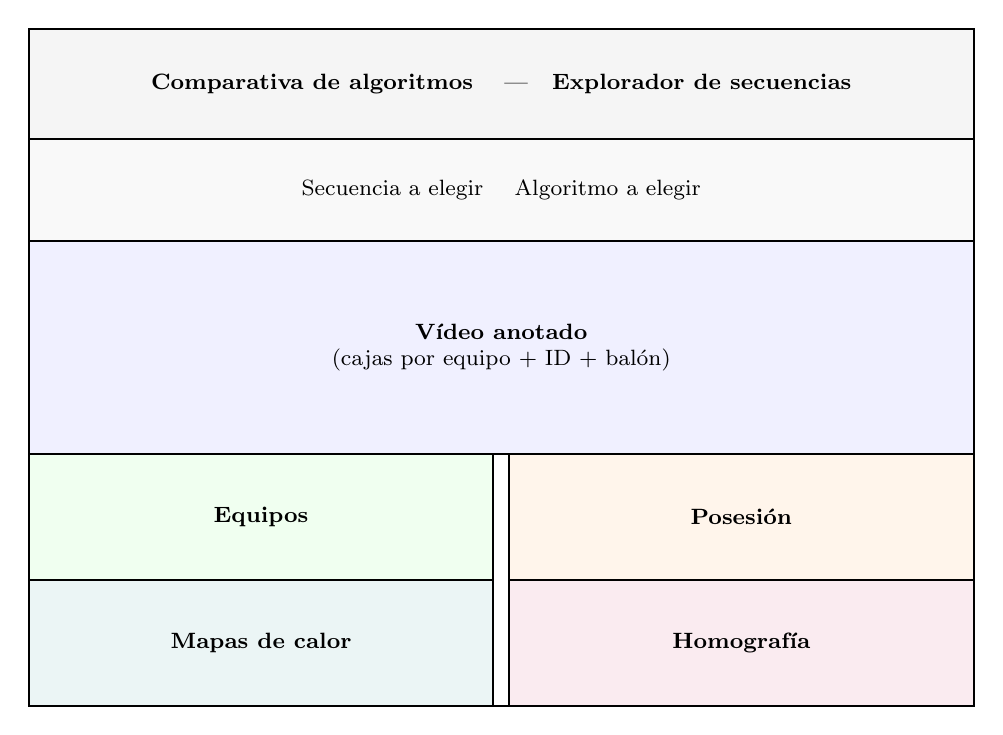
\begin{tikzpicture}[
  every node/.style={font=\footnotesize, align=center},
  panel/.style={draw, thick}
]
\draw[panel] (0,0) rectangle (12,8.6);
\draw[panel, fill=gray!8] (0,7.2) rectangle (12,8.6);
\node at (6,7.9) {\textbf{Comparativa de algoritmos} \quad|\quad \textbf{Explorador de secuencias}};
\draw[panel, fill=gray!5] (0,5.9) rectangle (12,7.2);
\node at (6,6.55) {Secuencia a elegir \quad Algoritmo a elegir};
\draw[panel, fill=blue!6] (0,3.2) rectangle (12,5.9);
\node at (6,4.55) {\textbf{Vídeo anotado}\\(cajas por equipo + ID + balón)};
\draw[panel, fill=green!6] (0,1.6) rectangle (5.9,3.2);
\node at (2.95,2.4) {\textbf{Equipos}};
\draw[panel, fill=orange!8] (6.1,1.6) rectangle (12,3.2);
\node at (9.05,2.4) {\textbf{Posesión}};
\draw[panel, fill=teal!8] (0,0) rectangle (5.9,1.6);
\node at (2.95,0.8) {\textbf{Mapas de calor}};
\draw[panel, fill=purple!8] (6.1,0) rectangle (12,1.6);
\node at (9.05,0.8) {\textbf{Homografía}};
\end{tikzpicture}
\caption{Croquis de la disposición implementada de la pestaña Explorador de secuencias}
\label{fig:diseno-web-wireframe}
\end{figure}
